\documentclass[dvipdfmx]{standalone}
\usepackage{circuitikz}
\begin{document}
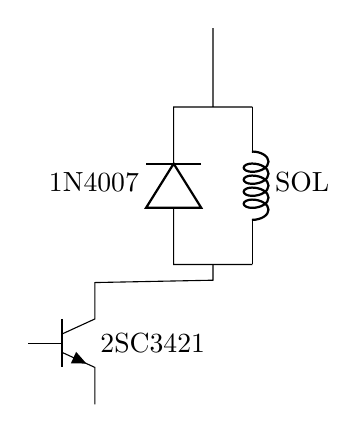
\begin{tikzpicture}
\draw (0,0) to [cute inductor=SOL] (0,-2);
\draw (0,-2)--(-1,-2) to [D,l=1N4007] (-1,0) --(0,0) (-0.5,0)--(-0.5,1);
\draw (-2,-3) node [npn,name=T1]{2SC3421};
\draw (-0.5,-2) --(-0.5,-2.2) to (T1.C);
\end{tikzpicture}
\end{document}